% Created 2018-10-30 Tue 10:57
% Intended LaTeX compiler: pdflatex
\documentclass[11pt, reqno, oneside]{amsbook}
              \newcommand\subtitle[1]{\newcommand\mrgsubtitle{#1}}
\newcommand\mrgproject{Torsten}
\newcommand\mrgtitle{Torsten: A Pharmacokinetic/Pharmacodynamic Model Library for Stan}
\newcommand\mrgsubtitle{\Large{User Manual} \linebreak (Torsten Version 0.85, Stan version 2.18.0)}
\renewcommand\maketitle{
  \begin{titlepage}%
    \definecolor{MRGGreen}{rgb}{0, 0.350, 0.200}

    \thispagestyle{empty}

    \begin{center}
      
\includegraphics[height=0.75in]{graphics/logo.jpg}\\
      \vspace{10mm} %5mm vertical space
      \textcolor{MRGGreen}{\sf Metrum Research Group LLC \hfill 2 Tunxis Road, Suite 112} \\
      \textcolor{MRGGreen}{\sf Phone: 860.735.7043 \hfill Tariffville, CT 06081}\\
      \textcolor{MRGGreen}{\sf billg@metrumrg.com \hfill \href{http://www.metrumrg.com/}{www.metrumrg.com}}\\
      {\Huge \textcolor{MRGGreen}{\textbf{\mrgproject}} \\ \ \\  \huge{\mrgtitle} \\ \ \\ \mrgsubtitle\\ \ \\ \ \\
        
        \large February 2018}
    \end{center}

    \clearpage
  \end{titlepage}%
}

\usepackage{imakeidx}
\makeindex
\usepackage[letterpaper, width=6.5in, height=9in]{geometry}
\usepackage{graphicx}
\usepackage{pdfpages}
\usepackage{amssymb}
\usepackage{epstopdf}
\usepackage{xcolor}
\definecolor{MRGGreen}{rgb}{0, 0.350, 0.200}
\usepackage[colorlinks=true, citecolor=MRGGreen, urlcolor=MRGGreen, linkcolor=MRGGreen]{hyperref}
\usepackage{courier}
\usepackage{listings}
\usepackage{siunitx}
\usepackage{booktabs}
\usepackage[framemethod=TikZ, skipabove=10pt, skipbelow=10pt, backgroundcolor=black!5, roundcorner=4pt, linewidth=1pt]{mdframed}
\BeforeBeginEnvironment{minted}{\begin{mdframed}}
\AfterEndEnvironment{minted}{\end{mdframed}}
\usepackage{subcaption}
\renewcommand{\chaptername}{}
\numberwithin{section}{chapter}
\theoremstyle{remark}
\newtheorem{example}{Example}
\newtheorem{remark}{Remark}


\usepackage[utf8]{inputenc}
\usepackage[T1]{fontenc}
\usepackage{graphicx}
\usepackage{grffile}
\usepackage{longtable}
\usepackage{wrapfig}
\usepackage{rotating}
\usepackage[normalem]{ulem}
\usepackage{amsmath}
\usepackage{textcomp}
\usepackage{amssymb}
\usepackage{capt-of}
\usepackage{hyperref}
\usepackage[newfloat]{minted}
\usepackage{caption}
\setcounter{secnumdepth}{3}
\author{Yi Zhang}
\date{\today}
\title{Torsten: A Pharmacokinetic/Pharmacodynamic Model Library for Stan\\\medskip
\large User Manual \\  (Torsten Version 0.85, Stan version 2.18.0)}
\hypersetup{
 pdfauthor={Yi Zhang},
 pdftitle={Torsten: A Pharmacokinetic/Pharmacodynamic Model Library for Stan},
 pdfkeywords={},
 pdfsubject={},
 pdfcreator={Emacs 25.3.1 (Org mode 9.1.3)}, 
 pdflang={English}}
\begin{document}

\maketitle
\tableofcontents


\section*{Development team}
\label{sec:org93dd0de}
\subsection*{Bill Gillespie}
\label{sec:org7a29b6b}
\href{mailto:billg@metrumrg.com}{\texttt{billg@metrumrg.com}},
Metrum Research Group, LLC
\subsection*{Yi Zhang}
\label{sec:org42df14b}
\href{mailto:yiz@metrumrg.com}{\texttt{yiz@metrumrg.com}}, Metrum Research Group, LLC
\subsection*{Charles Margossian}
\label{sec:org713c304}
\href{mailto:charles.margossian@columbia.edu}{\texttt{charles.margossian@columbia.edu}}, Columbia University, Department of Statistics(formerly Metrum Research Group, LLC)

\chapter*{Acknowledgements}
\label{sec:orgee5ef1a}
\section*{Institutions}
\label{sec:orga9f2273}
We thank Metrum Research Group, Columbia University, and AstraZeneca.
\section*{Funding}
\label{sec:org57a68fd}
This work was funded in part by the following organizations:
\subsection*{Office of Naval Research (ONR) contract N00014-16-P-2039}
\label{sec:org3ba4a5a}
provided as part of the Small Business Technology Transfer (STTR)
program. The content of the information presented in this document
does not necessarily reflect the position or policy of the
Government and no official endorsement should be inferred.
\subsection*{Bill \& Melinda Gates Foundation.}
\label{sec:orgee1a7d5}
\section*{Individuals}
\label{sec:org2ba29ba}
We thank the Stan Development Team for giving us guidance on how to
create new Stan functions and adding features to Stan's core language
that facilitate building ODE-based models.

We also thank Kyle Baron and Hunter Ford for helpful advice on coding
in C++ and using GitHub, Curtis Johnston for reviewing the User
Manual, and Yaming Su for using Torsten and giving us feedback.

\chapter{Introduction}
\label{sec:orge651e88}
Stan is an open source probabilistic programing language designed
primarily to do Bayesian data analysis \cite{carpenter17_stan}. Several of its
features make it a powerful tool to specify and fit complex
models. Notably, its language is extremely flexible and its No U-Turn
Sampler (NUTS), an adaptative Hamiltonian Monte Carlo algorithm, has
proven more efficient than commonly used Monte Carlo Markov Chains
(MCMC) samplers for complex high dimensional problems \cite{hoffman_no-u-turn_2011}. Our
goal is to harness these innovative features and make Stan a better
software for pharmacometrics modeling. Our efforts are twofold:
\begin{enumerate}
\item We contribute to the development of new mathematical tools, such as functions that support differential equations based models, and implement them directly into Stan's core language.
\item We develop Torsten, an extension with specialized pharmacometrics functions.
\end{enumerate}

Throughout the process, we work very closely with the Stan Development
Team. We have benefited immensely from their mentorship, advice, and
feedback. Just like Stan, Torsten is an open source project that
fosters collaborative work. Interested in contributing? Shoot us an
e-mail and we will help you help us(\href{mailto:billg@metrumrg.com}{billg@metrumrg.com})!

Torsten is licensed under the BSD 3-clause license.

\begin{mdframed}
\textbf{WARNING:} The current version of Torsten is a \emph{prototype}. It
is being released for review and comment, and to support limited
research applications. It has not been rigorously tested and should
not be used for critical applications without further testing or
cross-checking by comparison with other methods.

We encourage interested users to try Torsten out and are happy to
assist. Please report issues, bugs, and feature requests on
\href{https://github.com/metrumresearchgroup/stan}{our GitHub page}.
\end{mdframed}

\section{Overview}
\label{sec:org9895a22}
Torsten is a collection of Stan functions to facilitate analysis of
pharmacometric data using Stan. The current version
includes:
\begin{itemize}
\item Specific linear compartment models:
\begin{itemize}
\item One compartment model with first order absorption.
\item Two compartment model with elimination from and first order absorption into central compartment
\end{itemize}
\item General linear compartment model described by a system of first-order \underline{linear} Ordinary Differential Equations (ODEs).
\item General compartment model described by a system of first order ODEs.
\item Mix compartment model with PK forcing function described by a linear one or two compartment model.
\end{itemize}

The models and data format are based on
NONMEM\textregistered{}\footnote{NONMEM\textregistered{} is licensed and distributed by ICON Development Solutions.}/NMTRAN/PREDPP
conventions including:
\begin{itemize}
\item Recursive calculation of model predictions
\begin{itemize}
\item This permits piecewise constant covariate values
\end{itemize}
\item Bolus or constant rate inputs into any compartment
\item Handles single dose and multiple dose histories
\item Handles steady state dosing histories
\begin{itemize}
\item Note: The infusion time must be shorter than the inter-dose interval.
\end{itemize}
\item Implemented NMTRAN data items include: TIME, EVID, CMT, AMT, RATE, ADDL, II, SS
\end{itemize}

In general, all real variables may be passed as Stan parameters. A
few exceptions apply /to functions which use a numerical
integrator/(i.e. the general and the mix compartment
models). The below listed cases present technical difficulties, which we expect to
overcome in Torsten's next release:
\begin{itemize}
\item In the case of a multiple truncated infusion rate dosing regimen:
\begin{itemize}
\item The bioavailability (F) and the amount (AMT) must be fixed.
\end{itemize}
\end{itemize}

This library provides Stan language functions that calculate amounts
in each compartment, given an event schedule and an ODE system.

\section{Implementation summary}
\label{sec:org14031cc}
\begin{itemize}
\item Current v0.85 Torsten is based on Stan v2.18.1.
\item All functions are programmed in C++ and are compatible
with the Stan math automatic differentiation library \cite{carpenter15_stan_math_librar}
\item One and two compartment models are based on analytical solutions of governing ODEs.
\item General linear compartment models are based on semi-analytical solutions using the built-in matrix exponential function
\item General compartment models are solved numerically using built-in ODE integrators in Stan. The tuning parameters of the solver are adjustable. The steady state solution is calculated using a numerical algebraic solver.
\item A mix compartment model's PK forcing function is solved
analytically, and its forced ODE system is solved
numerically.
\end{itemize}

\section{Development plans}
\label{sec:org5953e5c}
Our current plans for future development of Torsten include the
following:
\begin{itemize}
\item Build a system to easily share packages of Stan functions
(written in C++ or in the Stan language)
\item Allow numerical methods to handle
bioavailability fraction (F) as parameters in all cases.
\item Optimize Matrix exponential functions
\begin{itemize}
\item Function for the action of Matrix Exponential on a vector
\item Hand-coded gradients
\item Special algorithm for matrices with special properties
\end{itemize}
\item Fix issue that arises when computing the adjoint of the lag time
parameter (in a dosing compartment) evaluated at \(t_{\text{lag}} = 0\).
\item Extend formal tests
\begin{itemize}
\item We want more C++ Google unit tests to address cases users may
encounter
\item Comparison with simulations from the R package
\emph{mrgsolve} and the software NONMEM\textregistered{}
\item Recruit non-developer users to conduct beta testing
\end{itemize}
\end{itemize}

\section{Changelog}
\label{sec:orga86f1ec}
\subsection{0.85 \textit{<2018-10-20 Sat>}}
\label{sec:org5d7e371}
\begin{itemize}
\item Added
\label{sec:org770db48}
\begin{itemize}
\item Dosing rate as parameter
\end{itemize}
\item Changed
\label{sec:org1229810}
\begin{itemize}
\item Update with Stan version 2.18.0.
\end{itemize}
\end{itemize}

\subsection{0.84 \textit{<2018-02-24 Sat>}}
\label{sec:orgfcd6b4f}
\begin{itemize}
\item Added
\label{sec:org62f8d52}
\begin{itemize}
\item Piecewise linear interpolation function.
\item Univariate integral functions.
\end{itemize}

\item Changed
\label{sec:org442c8b2}
\begin{itemize}
\item Update with Stan version 2.17.1.
\item Minor revisions to User Manual.
\item Bugfixes.
\end{itemize}
\end{itemize}

\subsection{0.83 \textit{<2017-08-02 Wed>}}
\label{sec:orga123fbe}
\begin{itemize}
\item Added
\label{sec:org2186224}
\begin{itemize}
\item Work with TorstenHeaders
\item Each chain has a different initial estimate
\end{itemize}

\item Changed
\label{sec:org1f9e052}
\begin{itemize}
\item User manual
\item Fix misspecification in ODE system for TwoCpt example.
\item Other bugfixes
\end{itemize}
\end{itemize}


\subsection{0.82 \textit{<2017-01-29 Sun>}}
\label{sec:org0f8e4fa}
\begin{itemize}
\item Added
\label{sec:orgcff81e5}
\begin{itemize}
\item Allow parameter arguments to be passed as 1D or 2D arrays
\item More unit tests
\item Unit tests check automatic differentiation against finite differentiation.
\end{itemize}

\item Changed
\label{sec:orgab7f2bc}
\begin{itemize}
\item Split the parameter argument into three arguments: pMatrix
(parameters for the ODEs -- note: for linOdeModel, pMatrix
is replaced by the constant rate matrix K), biovar
(parameters for the biovariability), and tlag (parameters
for the lag time).
\item bugfixes
\end{itemize}
\end{itemize}

\subsection{0.81 \textit{<2016-09-27 Tue>}}
\label{sec:org83da4e5}
\begin{itemize}
\item Added
\label{sec:orge8a83b4}
linCptModel (linear compartmental model) function
\end{itemize}

\subsection{0.80a \textit{<2016-09-21 Wed>}}
\label{sec:org2e38cd0}
\begin{itemize}
\item Added
\label{sec:org56f6aa5}
check\(_{\text{finite}}\) statements in pred\(_{\text{1}}\) and pred\(_{\text{2}}\) to reject metropolis proposal if initial conditions are not finite
\end{itemize}




\chapter{Installation}
\label{sec:org6ac36bb}
We are working with Stan development team to create a
system to add and share Stan packages. In the mean time,
the current repo contains forked version of Stan with
Torsten. The latest version of Torsten (v0.85) is
compatible with Stan v2.18.1. Torsten is agnostic to which
Stan interface you use. Here we provide command line and R
interfaces.

After downloading the project 

\begin{itemize}
\item \url{https://github.com/metrumresearchgroup/Torsten}
\end{itemize}

to \texttt{torsten\_path}, set the envionment variable
\mintinline[breaklines=true,fontsize=\footnotesize,breakanywhere=true]{sh}{TORSTEN_PATH} as
\begin{minted}[breaklines=true,fontsize=\footnotesize,breakanywhere=true]{sh}
# in bash
export TORSTEN_PATH=torsten_path
# in csh
setenv TORSTEN_PATH torsten_path
\end{minted}

\subsection{Command line interface}
\label{sec:orgcc35e7c}
The command line interface \texttt{cmdstan} does not require
installation. The following command
builds a Torsten model \texttt{model\_name} in \texttt{model\_path}
\begin{minted}[breaklines=true,fontsize=\footnotesize,breakanywhere=true]{sh}
cd $TORSTEN_PATH/cmdstan; make model_path/model_name
\end{minted}

\subsection{R interface}
\label{sec:org0f8c70b}
The R interface is based on \href{https://cran.r-project.org/web/packages/rstan/index.html}{rstan}, the Stan's interface for
R. To install R version of Torsten, at \texttt{\$TORSTEN\_PATH}, in R
\begin{minted}[breaklines=true,fontsize=\footnotesize,breakanywhere=true]{r}
source('install.R')
\end{minted}

Please ensure the R toolchain includes a C++ compiler with
C++14 support. In particular, R 3.4.0 and later is
recommended as it contains toolchain based on gcc 4.9.3. On
Windows platform, such a toolchain can be found in Rtools34 and later.

Please ensure \texttt{.R/Makevars} constains the following flags
\begin{minted}[breaklines=true,fontsize=\footnotesize,breakanywhere=true]{sh}
CXXFLAGS=-O3 -std=c++1y -mtune=native -march=native -Wno-unused-variable -Wno-unused-function
CXXFLAGS += -DBOOST_MPL_CFG_NO_PREPROCESSED_HEADERS -DBOOST_MPL_LIMIT_LIST_SIZE=30

CXX14FLAGS=-O3 -std=c++1y -mtune=native -march=native -Wno-unused-variable -Wno-unused-function
CXX14FLAGS += -DBOOST_MPL_CFG_NO_PREPROCESSED_HEADERS -DBOOST_MPL_LIMIT_LIST_SIZE=30
\end{minted}

For more information of installation troubleshooting,
please consult \href{https://github.com/stan-dev/rstan/wiki}{rstan wiki}.

\subsection{Testing}
\label{sec:org1213039}
To test the installation, run
\begin{minted}[breaklines=true,fontsize=\footnotesize,breakanywhere=true]{sh}
./test-torsten.sh --unit        # math unit test
./test-torsten.sh --signature   # stan function # signature test
./test-torsten.sh --model       # R model test, takes long time to finish
\end{minted}

\chapter{Using Torsten}
\label{sec:org2f9cdb4}
The reader should have a basic understanding of how Stan works before
reading this chapter. There are excellent resources online to get
started with Stan

\begin{itemize}
\item \href{http://mc-stan.org/documentation}{http://mc-stan.org/documentation}
\end{itemize}


In this section we go through the different functions Torsten adds to
Stan. The code for the examples can be found at

\begin{itemize}
\item \href{https://github.com/metrumresearchgroup/example-models}{https://github.com/metrumresearchgroup/example-models}
\end{itemize}

\section{One Compartment Model}
\label{sec:org9463ee6}
\index{One Compartment Model}
\begin{minted}[breaklines=true,fontsize=\footnotesize,breakanywhere=true]{stan}
real[nt, ncmt] = PKModelOneCpt(real[] time, real[] amt, real[] ate,
                               real[] ii, int[] evid, int[] cmt,
                               real[] addl, int[] ss, real[] theta,
                               real[] biovar, real[] tlag)
\end{minted}
Torsten function \texttt{PKModelOneCpt} (see also Figure \ref{fig:orgfcb929c}) solves one-compartment PK
models. The model obtains plasma concentrations of parent drug \(c=y_2/V_2\)
by solving for the mass of drug in the central compartment
\(y_2\) from ordinary differential equations(ODEs)
\begin{align*}
  y_1' &= -k_a y_1, \\
  y_2' &= k_a y_1 - \left(\frac{CL}{V_2} + \frac{Q}{V_2}\right) y_2.
\end{align*}

\begin{itemize}
\item ODE Parameters \texttt{theta} consists of \(CL\), \(V_2\), \(k_a\), in that order.
\item The event arguments \texttt{time}, \texttt{amt}, \texttt{rate}, \texttt{ii}, \texttt{evid}, \texttt{cmt}, \texttt{addl}, and
\texttt{ss}, describe the event schedule of the clinical
trial. All arrays have the same length corresponding to the number of events.
\item The model arguments, other than \texttt{theta}, include
\begin{itemize}
\item \texttt{biovar}, the bioavailability fraction in each compartment
\item \texttt{tlag}, the lag time in each compartment.
\end{itemize}
\item \texttt{theta}, \texttt{biovar}, \texttt{tlag} may be either 
\begin{itemize}
\item one-dimensional array \mintinline[breaklines=true,fontsize=\footnotesize,breakanywhere=true]{stan}{real[]}
for constants of all events, or
\item two-dimensional array \mintinline[breaklines=true,fontsize=\footnotesize,breakanywhere=true]{stan}{real[ , ]}
so that the \(i\)th row of the array describes
the model arguments for time interval \((t_{i-1}, t_i)\),
and the number of the rows euqals to the number of events.
\end{itemize}
\item Setting \(k_a = 0\) eliminates the first-order absorption.
\item The function returns a two-dimensional array of size \texttt{nt}
by \texttt{ncmt}, where \texttt{nt} is the number of time steps and
\texttt{ncmt=2} is the number of compartments.
\end{itemize}

\section{Two Compartment Model}
\label{sec:org6d984e8}
\label{org13f3df1}
\begin{minted}[breaklines=true,fontsize=\footnotesize,breakanywhere=true]{stan}
real[nt, ncmt] = PKModelTwoCpt(real[] time, real[] amt, real[] ate,
                               real[] ii, int[] evid, int[] cmt,
                               real[] addl, int[] ss, real[] theta,
                               real[] biovar, real[] tlag)
\end{minted}

\begin{figure}[htbp]
\centering
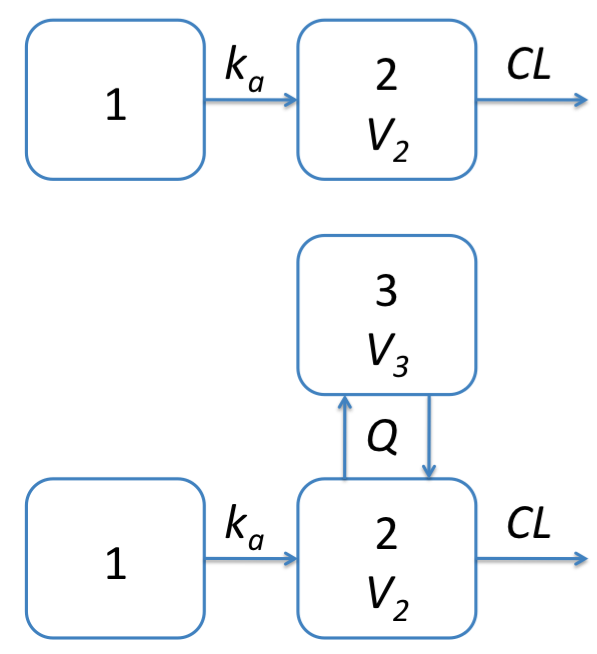
\includegraphics[width=2.0in]{./graphics/cptModels.png}
\caption{\label{fig:orgfcb929c}
One and two compartment models with first order absorption implemented in Torsten.}
\end{figure}

Torsten function \texttt{PKModelTwoCpt} (see also Figure \ref{fig:orgfcb929c}) solves two-compartment PK
models. The model obtains plasma concentrations of parent drug \(c=y_2/V_2\)
by solving for \(y_2\) and \(y_3\), the mass of drug in the central and peripheral compartments,
respectively, from ODEs
\begin{align} \label{eq:twocpt}
  y_1' &= -k_a y_1 \\
  y_2' &= k_a y_1 - \left(\frac{CL}{V_2} + \frac{Q}{V_2}\right) y_2 +  \frac{Q}{V_3}  y_3  \\ 
  y_3' &= \frac{Q}{V_2} y_2 - \frac{Q}{V_3} y_3
\end{align}

\begin{itemize}
\item ODE Parameters \texttt{theta} consists of \(CL\), \(Q\), \(V_2\), \(V_3\), \(k_a\).
\item The event arguments \texttt{time}, \texttt{amt}, \texttt{rate}, \texttt{ii}, \texttt{evid}, \texttt{cmt}, \texttt{addl}, and
\texttt{ss}, describe the event schedule of the clinical
trial. All arrays have the same length corresponding to the number of events.
\item See section \ref{orgea981de} regarding model arguments \texttt{theta},
\texttt{biovar}, and \texttt{tlag}.
\item Setting \(ka\) to 0 eliminates the first-order absorption.
\item The function returns a two-dimensional array of size \texttt{nt}
by \texttt{ncmt}, where \texttt{nt} is the number of time steps and
\texttt{ncmt=3} is the number of compartments.
\end{itemize}

\subsection{Example}
\label{sec:org1c6bfe5}
We model drug absorption in a single patient and simulate plasma drug concentrations:

\begin{itemize}
\item Multiple Doses: 1250 mg, every 12 hours, for a total of 15 doses
\item PK measured at 0.083, 0.167, 0.25, 0.5, 0.75, 1, 1.5, 2, 4, 6,
8, 10 and 12 hours after 1st, 2nd, and 15th dose. In addition, the
PK is measured every 12 hours throughout the trial.
\end{itemize}

With the plasma concentration \(\hat{c}\) solved from
two-compartment ODEs, we simulate \(c\) according to:
\begin{align*}
  \log\left(c\right) &\sim N\left(\log\left(\widehat{c}\right),\sigma^2\right) \\
  \left(CL, Q, V_2, V_3, ka\right) &= \left(5\ {\rm L/h}, 8\  {\rm L/h}, 20\  {\rm L},  70\ {\rm L}, 1.2\ {\rm h^{-1}} \right) \\
  \sigma^2 &= 0.01
\end{align*}
The data are generated using the R package \texttt{mrgsolve} \cite{Baron000}. 

Code below shows how Torsten function \texttt{PKModelTwoCpt} can be used to fit the above model.

\begin{minted}[breaklines=true,fontsize=\footnotesize,breakanywhere=true]{stan}
data{
  int<lower = 1> nt;  // number of events
  int<lower = 1> nObs;  // number of observation
  int<lower = 1> iObs[nObs];  // index of observation

  // NONMEM data
  int<lower = 1> cmt[nt];
  int evid[nt];
  int addl[nt];
  int ss[nt];
  real amt[nt];
  real time[nt];
  real rate[nt];
  real ii[nt];

  vector<lower = 0>[nObs] cObs;  // observed concentration (Dependent Variable)
}

transformed data{
  vector[nObs] logCObs = log(cObs);
  int nTheta = 5;  // number of ODE parameters in Two Compartment Model
  int nCmt = 3;  // number of compartments in model

  // Since we're not trying to evaluate the bio-variability (F) and 
  // the lag times, we declare them as data.
  real biovar[nCmt];
  real tlag[nCmt];

  biovar[1] = 1;
  biovar[2] = 1;
  biovar[3] = 1;

  tlag[1] = 0;
  tlag[2] = 0;
  tlag[3] = 0;

}

parameters{
  real<lower = 0> CL;
  real<lower = 0> Q;
  real<lower = 0> V1;
  real<lower = 0> V2;
  real<lower = 0> ka;
  real<lower = 0> sigma;

}

transformed parameters{
  real theta[nTheta];  // ODE parameters
  vector<lower = 0>[nt] cHat;
  vector<lower = 0>[nObs] cHatObs;
  matrix<lower = 0>[nt, nCmt] x; 

  theta[1] = CL;
  theta[2] = Q;
  theta[3] = V1;
  theta[4] = V2;
  theta[5] = ka;

  // PKModelTwoCpt takes in the NONMEM data, followed by the parameter
  // arrays abd returns a matrix with the predicted amount in each 
  // compartment at each event.
  x = PKModelTwoCpt(time, amt, rate, ii, evid, cmt, addl, ss,
                   theta, biovar, tlag);

  cHat = col(x, 2) ./ V1; // we're interested in the amount in the second compartment 

  cHatObs = cHat[iObs]; // predictions for observed data recors
\end{minted}

Three MCMC chains of 2000 iterations are simulated. The first
1000 iteration of each chain were discarded. Thus 1000 MCMC samples
per chain were used for the subsequent analyses.
The MCMC history plots(Figure \ref{fig:org0831756})
suggest that the 3 chains have converged to common distributions for
all of the key model parameters. The fit to the plasma concentration
data (Figure \ref{fig:orgd299842}) are in close agreement with the
data, which is not surprising since the fitted model is identical to
the one used to simulate the data. Similarly the parameter estimates
summarized in Table \ref{tab:org9a031e5} and Figure \ref{fig:orgcda0339}
are consistent with the values used for simulation.

\begin{table}[htbp]
\caption{\label{tab:org9a031e5}
Summary of the MCMC simulations of the marginal posterior distribu- tions of the model parameters}
\centering
\begin{tabular}{lrrrrrrrrrr}
\hline
 & mean & se\(_{\text{mean}}\) & sd & 2.5\% & 25\% & 50\% & 75\% & 97.5\% & n\(_{\text{eff}}\) & Rhat\\
\hline
CL & 4.823 & 0.002 & 0.092 & 4.647 & 4.762 & 4.823 & 4.883 & 5.012 & 2392.155 & 1.00\\
Q & 7.596 & 0.013 & 0.586 & 6.479 & 7.201 & 7.594 & 7.977 & 8.785 & 1923.939 & 1.00\\
V1 & 21.073 & 0.069 & 2.573 & 16.017 & 19.352 & 21.046 & 22.817 & 26.097 & 1385.883 & 1.00\\
V2 & 76.365 & 0.105 & 5.611 & 65.805 & 72.623 & 76.172 & 79.916 & 87.971 & 2862.184 & 1.00\\
ka & 1.231 & 0.004 & 0.177 & 0.907 & 1.107 & 1.221 & 1.344 & 1.599 & 1581.825 & 1.00\\
sigma & 0.109 & 0.000 & 0.012 & 0.089 & 0.100 & 0.108 & 0.116 & 0.134 & 2560.112 & 1.00\\
\hline
\end{tabular}
\end{table}

\begin{figure}[htbp]
\centering
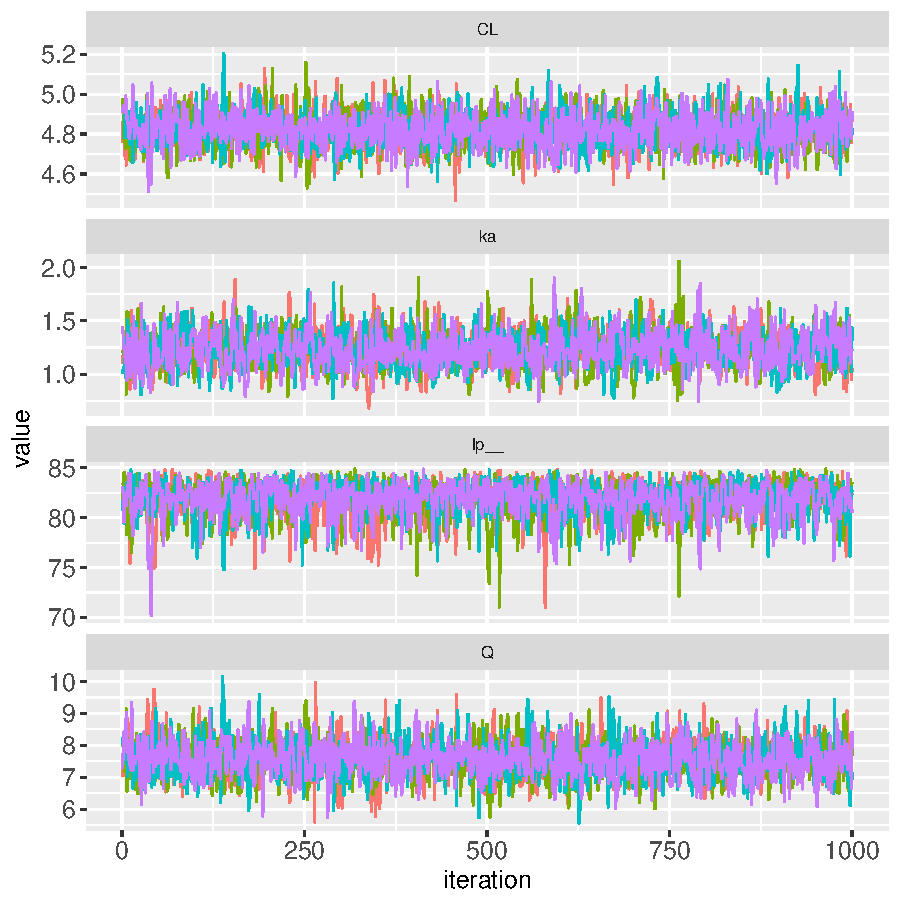
\includegraphics[width=0.6\linewidth]{../example-models/R/deliv/figure/TwoCptModel/TwoCptModelPlots001.pdf}
\caption{\label{fig:org0831756}
MCMC history plots for the parameters of a two compartment model with first order absorption (each color corresponds to a different chain)}
\end{figure}

\begin{figure}[htbp]
\centering
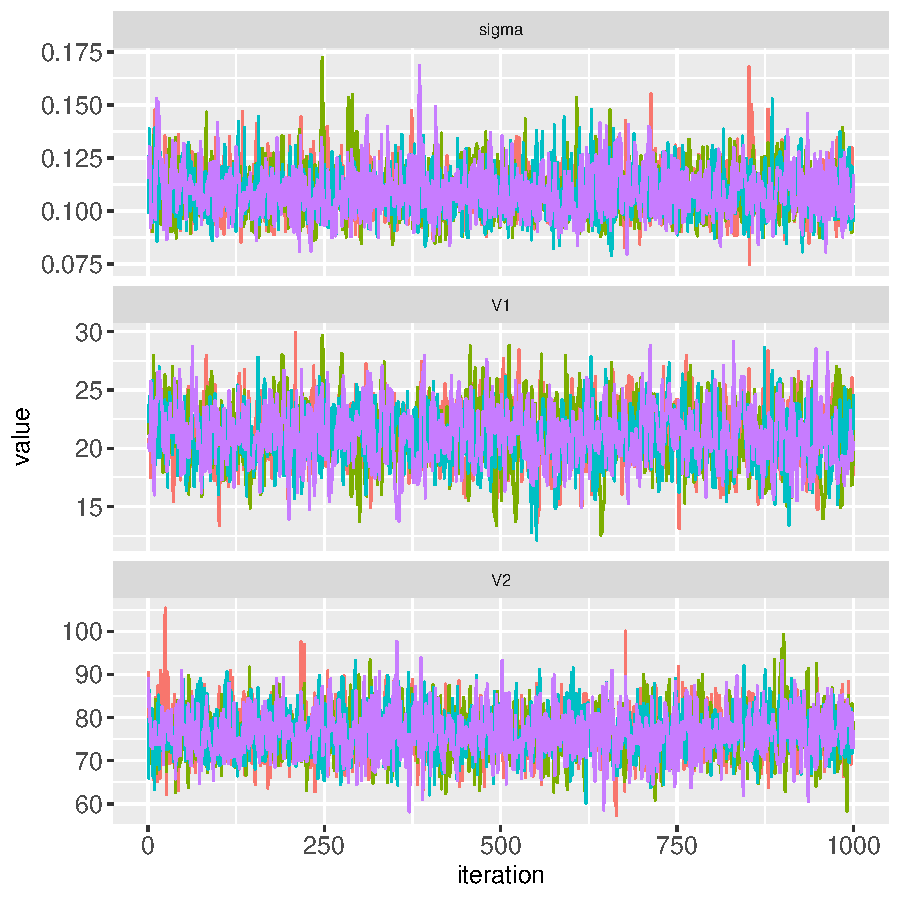
\includegraphics[width=0.6\linewidth]{../example-models/R/deliv/figure/TwoCptModel/TwoCptModelPlots002.pdf}
\caption{\label{fig:org63353c0}
MCMC history plots for the parameters of a two compartment model with first order absorption (each color corresponds to a different chain)}
\end{figure}

\begin{figure}[htbp]
\centering
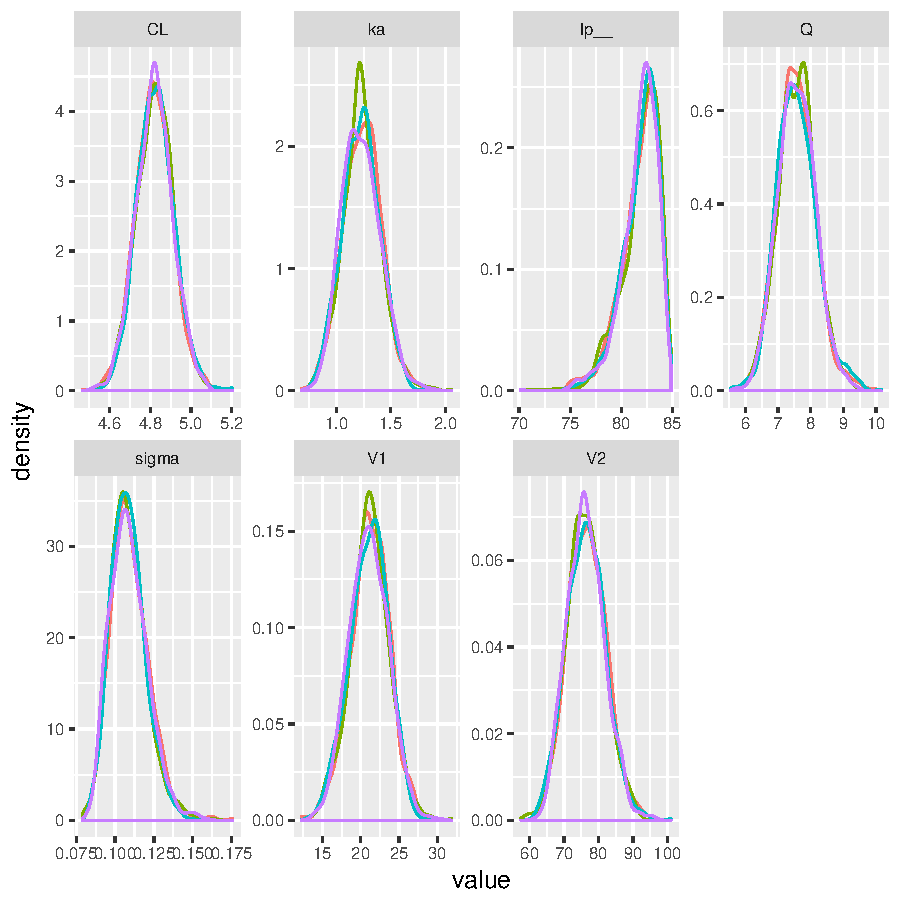
\includegraphics[width=0.6\linewidth]{../example-models/R/deliv/figure/TwoCptModel/TwoCptModelPlots003.pdf}
\caption{\label{fig:orgcda0339}
Posterior Marginal Densities of the Model Parameters of a two compartment model with first order absorption (each color corresponds to a different chain)}
\end{figure}

\begin{figure}[htbp]
\centering
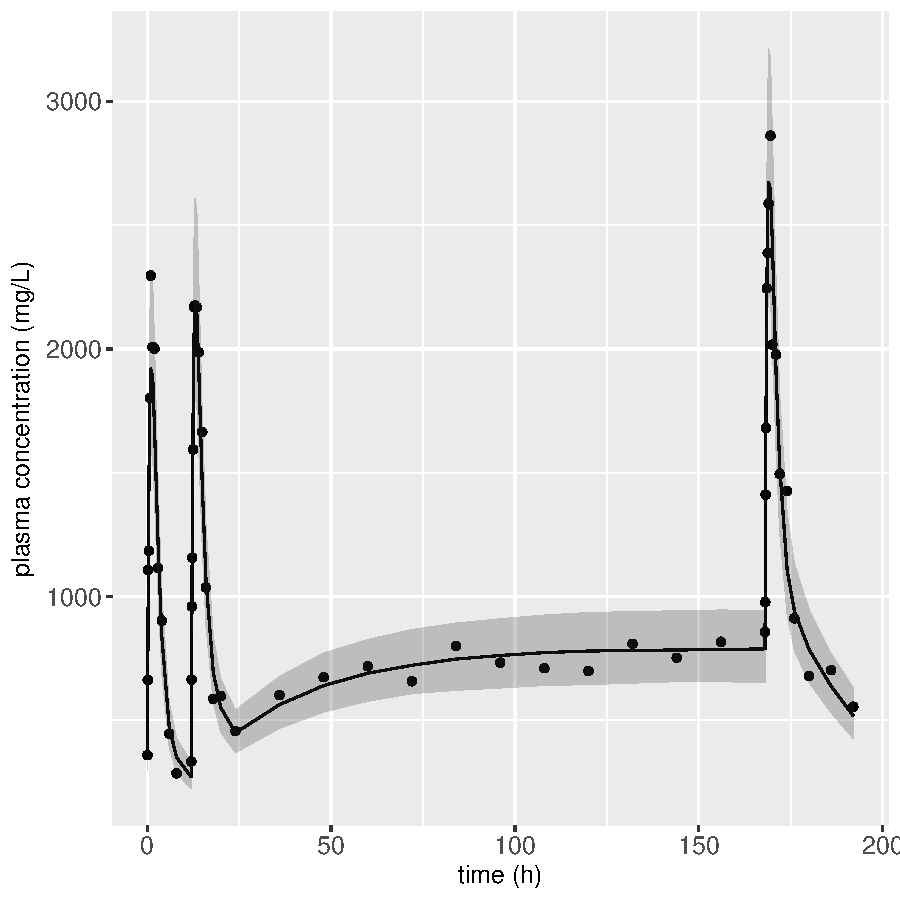
\includegraphics[width=0.6\linewidth]{../example-models/R/deliv/figure/TwoCptModel/TwoCptModelPlots006.pdf}
\caption{\label{fig:orgd299842}
Predicted (posterior median and 90\% credible intervals) and observed plasma drug concentrations of a two compartment model with first order absorption}
\end{figure}


\section{General Linear ODE Model Function}
\label{sec:orgb212f8b}
\index{General linear model}
\begin{minted}[breaklines=true,fontsize=\footnotesize,breakanywhere=true]{stan}
real[nt, n] = linOdeModel(real[] time, real[] amt, real[] rate,
                     real[] ii, int[] evid, int[] cmt,
                     real[] addl, int[] ss,
                     matrix K, real[] biovar, real[] tlag)
\end{minted}
Torsten function \texttt{linOdeModel} 
solves a (piecewise) linear ODEs model with coefficients
in form of matrix \(K\)
\begin{equation}
y^\prime\left(t\right) = Ky\left(t\right)
\end{equation}
For example, for a two-compartment
model with first order absorption, \(K\) would be
\begin{equation}
  K = \left[\begin{array}{ccc}
              -k_a & 0 & 0 \\
              k_a & -\left(k_{10} + k_{12}\right) & k_{21} \\
              0 & k_{12} & -k_{21}
            \end{array}\right]
\end{equation}
where \(k_{10}=CL/V_2\), \(k_{12}=Q/V_2\), and \(k_{21}=Q/V_3\).

\begin{itemize}
\item \texttt{K} contains system parameters. In the case of constant rate,
\end{itemize}
\texttt{K} is the same for all events or an array of constant rate
matrices. The length of the array is
the number of events and the \texttt{i} th element corresponds to the matrix at
the interval \texttt{[ time[i-1], time[i] ]}.
Note that \texttt{K} contains all the ODE parameters, so we no
longer need \texttt{theta}.
\begin{itemize}
\item See section \ref{orgea981de} regarding model arguments \texttt{theta},
\texttt{biovar}, and \texttt{tlag}.
\item The function returns a two-dimensional array of size \texttt{nt}
by \texttt{n}, where \texttt{nt} is the number of time steps and
\texttt{n} is the size of the square matrix \texttt{K}.
\end{itemize}

\subsection{Example}
\label{sec:org24950a9}
Using \texttt{linOdeModel}, the following example fits a two-compartment model
with first order absorption.

\begin{minted}[breaklines=true,fontsize=\footnotesize,breakanywhere=true]{stan}
// LinTwoCptModelExample.stan
// Run two compartment model using matrix exponential solution
// Heavily anotated to help new users

data{
  int<lower = 1> nt;  // number of events
  int<lower = 1> nObs;  // number of observations
  int<lower = 1> iObs[nObs];  // index of observation

  // NONMEM data
  int<lower = 1> cmt[nt];
  int evid[nt];
  int addl[nt];
  int ss[nt];
  real amt[nt];
  real time[nt];
  real rate[nt];
  real ii[nt];

  vector<lower = 0>[nObs] cObs;  // observed concentration (dependent variable)
}

transformed data{
  vector[nObs] logCObs = log(cObs);
  int nCmt = 3;
  real biovar[nCmt];
  real tlag[nCmt];

  for (i in 1:nCmt) {
    biovar[i] = 1;
    tlag[i] = 0;
  }
}

parameters{
  real<lower = 0> CL;
  real<lower = 0> Q;
  real<lower = 0> V1;
  real<lower = 0> V2;
  real<lower = 0> ka;
  real<lower = 0> sigma;

}

transformed parameters{
  matrix[3, 3] K;
  real k10 = CL / V1;
  real k12 = Q / V1;
  real k21 = Q / V2;
  vector<lower = 0>[nt] cHat;
  vector<lower = 0>[nObs] cHatObs;
  matrix<lower = 0>[nt, 3] x;

  K = rep_matrix(0, 3, 3);

  K[1, 1] = -ka;
  K[2, 1] = ka;
  K[2, 2] = -(k10 + k12);
  K[2, 3] = k21;
  K[3, 2] = k12;
  K[3, 3] = -k21;

  // linModel takes in the constant rate matrix, the object theta which
  // contains the biovariability fraction and the lag time of each compartment,
  // and the NONMEM data.
  x = linOdeModel(time, amt, rate, ii, evid, cmt, addl, ss,
                  K, biovar, tlag);
\end{minted}

\section{General ODE Model Function}
\label{sec:org7012732}
\index{General ODE Model}
\begin{minted}[breaklines=true,fontsize=\footnotesize,breakanywhere=true]{stan}
real[] generalOdeModel_rk45(ODE_system, int nCmt,
                            real[] time, real[] amt, real[] rate, real[] ii,
                            int[] evid, int[] cmt, real[] addl, int[] ss,
                            real[] theta, real[] biovar, real[] tlag,                      
                            real rel_tol, real abs_tol, int max_step);
\end{minted}
\begin{minted}[breaklines=true,fontsize=\footnotesize,breakanywhere=true]{stan}
real[] generalOdeModel_bdf(ODE_system, int nCmt,
                           real[] time, real[] amt, real[] rate, real[] ii,
                           int[] evid, int[] cmt, real[] addl, int[] ss,
                           real[] theta, real[] biovar, real[] tlag,                      
                           real rel_tol, real abs_tol, int max_step);
\end{minted}
Torsten function \texttt{generalOdeModel\_rk45} and
\texttt{generalOdeModel\_bdf} solve first ODEs with
user-specified first-order right-hand-side(RHS)
\begin{equation*}
y'(t) = f(t, y(t))
\end{equation*}
In the case where the \texttt{rate} vector \(r\) is non-zero, this equation becomes:
\begin{equation*}
y'(t) = f(t, y(t)) + r
\end{equation*}

\begin{itemize}
\item User specifies \(f(t, y(t))\) by defining \texttt{ODE\_system}
\end{itemize}
inside the \texttt{functions} block (see section 19.2 of the
Stan reference manual for details and Figure\textasciitilde{}\ref{GenTwoCptModelCode}
for an example). The user does NOT include the rates in their
definition of \(f\). Torsten automatically corrects the derivatives when
the rates are non-zero.
\begin{itemize}
\item \texttt{nCmt} is the number of compartments (or, equivalently, the
\end{itemize}
number of ODEs) in the model. 
\begin{itemize}
\item \texttt{rel\_tol}, \texttt{abs\_tol},
\end{itemize}
and \texttt{max\_step} are tuning parameters for the ODE integrator:
respectively the relative tolerance, the absolute tolerance, and the
maximum number of steps.
\begin{itemize}
\item \texttt{generalOdeModel\_rk45} solves ODEs with Stan's Runge-Kutta
ODE solver function \texttt{integrate\_ode\_rk45}.
\item \texttt{generalOdeModel\_rk45} solves ODEs with Stan's Backward
Differentiation(BDF) ODE solver function \texttt{integrate\_ode\_bdf},
\item The values to use for the tuning parameters depends on the integrator and
the specifics of the ODE system. Reducing the tolerance parameters and
increasing the number of steps make for a more robust integrator but
can significantly slow down the algorithm. The following can be used
as a starting point: 
\begin{itemize}
\item \texttt{rel\_tol = 1e-6}
\item \texttt{abs\_tol = 1e-6}
\item \texttt{max\_step = 1e+6}
\end{itemize}
for rk45 integrator and
\begin{itemize}
\item \texttt{rel\_tol = 1e-10}
\item \texttt{abs\_tol = 1e-10}
\item \texttt{max\_step = 1e+8}
\end{itemize}
for the BDF integrator \footnote{These are the default tuning parameters the integrators. Torsten functions do not have a default values for these parameters. The user must explicitly pass the tuning parameters to \texttt{generalOdeModel\_*()} .}.
Users should be prepared to adjust these
values. For additional information, see the Stan User's
Manual \cite{stan_team_2017}.
\item In the case of a multiple truncated infusion rate dosing regimen
The bioavailability \texttt{biovar} and the amount \texttt{amt} cannot be passed as parameters.
\item See section \ref{orgea981de} regarding model arguments \texttt{theta},
\texttt{biovar}, and \texttt{tlag}.
\end{itemize}

\subsection{Example}
\label{sec:org1a9f821}
Using \texttt{generalOdeModel\_rk45}, the following example fits a two-compartment model
with first order absorption. User-defined function
\texttt{twoCptModelODE} describes the RHS of the ODEs.

\begin{minted}[breaklines=true,fontsize=\footnotesize,breakanywhere=true]{stan}
// GenTwoCptModelExample.stan
// Run two compartment model using numerical solution
// Heavily anotated to help new users

functions{

  // define ODE system for two compartmnt model
  real[] twoCptModelODE(real t,
                        real[] x,
                        real[] parms,
                        real[] rate,  // in this example, rate is treated as data
                        int[] dummy){

    // Parameters
    real CL = parms[1];
    real Q = parms[2];
    real V1 = parms[3];
    real V2 = parms[4];
    real ka = parms[5];

    // Re-parametrization
    real k10 = CL / V1;
    real k12 = Q / V1;
    real k21 = Q / V2;

    // Return object (derivative)
    real y[3];  // 1 element per compartment of
                // the model

    // PK component of the ODE system
    y[1] = -ka*x[1];
    y[2] = ka*x[1] - (k10 + k12)*x[2] + k21*x[3];
    y[3] = k12*x[2] - k21*x[3];

    return y;
  }

}
data{
  int<lower = 1> nt;  // number of events
  int<lower = 1> nObs;  // number of observations
  int<lower = 1> iObs[nObs];  // index of observation

  // NONMEM data
  int<lower = 1> cmt[nt];
  int evid[nt];
  int addl[nt];
  int ss[nt];
  real amt[nt];
  real time[nt];
  real rate[nt];
  real ii[nt];

  vector<lower = 0>[nObs] cObs;  // observed concentration (dependent variable)
}

transformed data{
  vector[nObs] logCObs = log(cObs);
  int nTheta = 5;   // number of parameters
  int nCmt = 3;   // number of compartments
  real biovar[nCmt];
  real tlag[nCmt];

  for (i in 1:nCmt) {
    biovar[i] = 1;
    tlag[i] = 0;
  }
}

parameters{
  real<lower = 0> CL;
  real<lower = 0> Q;
  real<lower = 0> V1;
  real<lower = 0> V2;
  real<lower = 0> ka;
  real<lower = 0> sigma;
}

transformed parameters{
  real theta[nTheta];
  vector<lower = 0>[nt] cHat;
  vector<lower = 0>[nObs] cHatObs;
  matrix<lower = 0>[nt, 3] x; 

  theta[1] = CL;
  theta[2] = Q;
  theta[3] = V1;
  theta[4] = V2;
  theta[5] = ka;

  // generalCptModel takes in the ODE system, the number of compartment 
  // (here we have a two compartment model with first order absorption, so
  // three compartments), the parameters matrix, the NONEM data, and the tuning
  // parameters (relative tolerance, absolute tolerance, and maximum number of steps)
  // of the ODE integrator. The user can choose between the bdf and the rk45 integrator.
  // Returns a matrix with the predicted amount in each compartment 
  // at each event.

//  x = generalOdeModel_bdf(twoCptModelODE, 3,
//                          time, amt, rate, ii, evid, cmt, addl, ss,
//                          theta, biovar, tlag,
//                          1e-8, 1e-8, 1e8);

   x = generalOdeModel_rk45(twoCptModelODE, 3,
                           time, amt, rate, ii, evid, cmt, addl, ss,
                           theta, biovar, tlag,
                           1e-6, 1e-6, 1e6);

  cHat = col(x, 2) ./ V1;

  for(i in 1:nObs){
    cHatObs[i] = cHat[iObs[i]];  // predictions for observed data records
  }
}
\end{minted}

\section{Mixed ODE Model Function}
\label{sec:orgf88ec75}
\index{Mixed ODE Model}

\begin{minted}[breaklines=true,fontsize=\footnotesize,breakanywhere=true]{stan}
real[] mixOde1CptModel_rk45(reduced_ODE_system, int nOde,
                            real[] time, real[] amt, real[] rate,
                            real[] ii, int[] evid, int[] cmt, real[]
                            addl, int[] ss,
                            real[] theta, real[] biovar, real[] tlag,
                            real rel_tol, real abs_tol, real max_step)
\end{minted}
\begin{minted}[breaklines=true,fontsize=\footnotesize,breakanywhere=true]{stan}
real[] mixOde1CptModel_bdf(reduced_ODE_system, int nOde,
                            real[] time, real[] amt, real[] rate,
                            real[] ii, int[] evid, int[] cmt, real[]
                            addl, int[] ss,
                            real[] theta, real[] biovar, real[] tlag,
                            real rel_tol, real abs_tol, real max_step)
\end{minted}
\begin{minted}[breaklines=true,fontsize=\footnotesize,breakanywhere=true]{stan}
real[] mixOde2CptModel_rk45(reduced_ODE_system, int nOde,
                            real[] time, real[] amt, real[] rate,
                            real[] ii, int[] evid, int[] cmt, real[]
                            addl, int[] ss,
                            real[] theta, real[] biovar, real[] tlag,
                            real rel_tol, real abs_tol, real max_step)
\end{minted}
\begin{minted}[breaklines=true,fontsize=\footnotesize,breakanywhere=true]{stan}
real[] mixOde2CptModel_bdf(reduced_ODE_system, int nOde,
                            real[] time, real[] amt, real[] rate,
                            real[] ii, int[] evid, int[] cmt, real[]
                            addl, int[] ss,
                            real[] theta, real[] biovar, real[] tlag,
                            real rel_tol, real abs_tol, real max_step)
\end{minted}
When the ODE system consists of two subsystems in form of
\begin{align*}
  y_1^\prime &= f_1(t, y_1), \\
  y_2^\prime &= f_2(t, y_1, y_2),
\end{align*}
with \(y_1\), \(y_2\), \(f_1\), and \(f_2\) being vector-valued functions, and
\(y_1^\prime\) independent of \(y_2\), the solution can be
accelerated if \(y_1\) admits an analytical solution which can
be introduced into the ODE for \(y_2\) for numerical
integration. This structure arises in PK/PD
models, where \(y_1\) describes a forcing PK function and \(y_2\) the PD
effects. In the example of a Friberg-Karlsson
semi-mechanistic model(see below), we observe an average speedup of
\(\sim 47 \pm 18 \%\) when using the mix solver in lieu of the numerical
integrator. Torsten supports the mixed solver for
cases where \(y_1\) solves the ODEs for a One or Two Compartment model
with a first-order absorption.

The \texttt{reduced\_ODE\_system} specifies the system we
numerically solve (\(y_2\) in the above discussion, also called the
\emph{reduced system} and \texttt{nOde} the number of equations in
the \underline{reduced} system. The function that defines a reduced
system has an almost identical signature to that used for a full
system, but takes one additional argument: \(y_1\), the PK states,
i.e. solution to the PK ODEs.
\begin{minted}[breaklines=true,fontsize=\footnotesize,breakanywhere=true]{stan}
real[] reducedODE(real t,       // time
                  real[] y,     // reduced state
                  real[] y1,    // PK states
                  real[] theta, // parameters
                  real[] x_r,   // data (real)
                  int[] x_int)  // data (integer)
\end{minted}

The four functions of mixed solver correspond to all the permutations Torsten
provides when using a forcing One or Two Compartment function, and the
Runge-Kutta 4th/5th order (\texttt{rk45}) or Backward Differentiation (\texttt{bdf})
integration scheme. The mixed ODE functions can be used to compute the
steady state solutions supported by the general ODE model functions.

Restrictions regarding which arguments may be passed as parameters for
general ODE solvers also apply to
mixed solvers.

\section{Example}
\label{sec:orgafa7501}
\index{Friberg-Karlsson Model}

A Friberg-Karlsson Semi-Mechanistic model \cite{friberg_mechanistic_2003} couples
a PK model with a PD
effect. In the current example, we use the two compartment model in section \ref{org13f3df1} for
PK model.

Neutropenia is observed in patients receiving an ME-2 drug. Our goal
is to model the relation between neutrophil counts and drug
exposure. Using a feedback mechanism, the body maintains the number of
neutrophils at a baseline value (Figure\textasciitilde{}\ref{FK}). While in the
patient's blood, the drug impedes the production of neutrophils. As a
result, the neutrophil count goes down. After the drug clears out, the
feedback mechanism kicks in and brings the neutrophil count back to
baseline.

\begin{align}
  \log(ANC_i) \sim& N(\log(Circ), \sigma^2_{ANC})  \\
  Circ =& f_{FK}(MTT, Circ_{0}, \alpha, \gamma, c)  \\
  (MTT, Circ_{0}, \alpha, \gamma, ktr) =& (125, 5.0, 3 \times 10^{-4}, 0.17) \\
  \sigma^2_{ANC} =& 0.001
\end{align}
where \(c\) is the drug concentration in the blood we get from the Two
Compartment model, and \(Circ\) is obtained by solving the following
system of nonlinear ODEs:

\begin{align}
 y_\mathrm{prol}' &= k_\mathrm{prol} y_\mathrm{prol} (1 - E_\mathrm{drug})\left(\frac{Circ_0}{y_\mathrm{circ}}\right)^\gamma - k_\mathrm{tr}y_\mathrm{prol} \\
 y_\mathrm{trans1}' &= k_\mathrm{tr} y_\mathrm{prol} - k_\mathrm{tr} y_\mathrm{trans1} \\
 y_\mathrm{trans2}' &= k_\mathrm{tr} y_\mathrm{trans1} - k_\mathrm{tr} y_\mathrm{trans2}  \\
 y_\mathrm{trans3}' &= k_\mathrm{tr} y_\mathrm{trans2} - k_\mathrm{tr} y_\mathrm{trans3}  \\
 y_\mathrm{circ}' &= k_\mathrm{tr} y_\mathrm{trans3} - k_\mathrm{tr} y_\mathrm{circ}
 \end{align}
   \label{eq:FK}
where \(E_{drug}  = \alpha c\).

The ODEs specifying the Two Compartment Model
(Equation \eqref{eq:twocpt}) do not depend on the PD ODEs
(Equation \eqref{eq:FK}) and can be solved analytically
using Torsten's \mintinline[breaklines=true,fontsize=\footnotesize,breakanywhere=true]{stan}{PKModelTwoCpt} function. We
therefore specify our model using a mixed solver function. We do not
expect our system to be stiff and use the Runge-Kutta 4th/5th order
integrator (Figures \ref{FK_reduced} and \ref{FK_mix2}).

\begin{minted}[breaklines=true,fontsize=\footnotesize,breakanywhere=true]{stan}
functions{
  real[] FK_ODE(real t,
                real[] y,
                real[] y_pk,
                real[] theta,
                real[] rdummy,
                int[] idummy){
    /* PK variables */
    real VC = theta[3];

    /* PD variable */
    real mtt      = theta[6];
    real circ0    = theta[7];
    real alpha    = theta[8];
    real gamma    = theta[9];
    real ktr      = 4.0 / mtt;
    real prol     = y[1] + circ0;
    real transit1 = y[2] + circ0;
    real transit2 = y[3] + circ0;
    real transit3 = y[4] + circ0;
    real circ     = fmax(machine_precision(), y[5] + circ0);
    real conc     = y_pk[2] / VC;
    real EDrug    = alpha * conc;

    real dydt[5];

    dydt[1] = ktr * prol * ((1 - EDrug) * ((circ0 / circ)^gamma) - 1);
    dydt[2] = ktr * (prol - transit1);
    dydt[3] = ktr * (transit1 - transit2);
    dydt[4] = ktr * (transit2 - transit3);
    dydt[5] = ktr * (transit3 - circ);

    return dydt;
  }
}

data{
  int<lower = 1> nt;
  int<lower = 1> nObsPK;
  int<lower = 1> nObsPD;
  int<lower = 1> iObsPK[nObsPK];
  int<lower = 1> iObsPD[nObsPD];
  real<lower = 0> amt[nt];
  int<lower = 1> cmt[nt];
  int<lower = 0> evid[nt];
  real<lower = 0> time[nt];
  real<lower = 0> ii[nt];
  int<lower = 0> addl[nt];
  int<lower = 0> ss[nt];
  real rate[nt];
  vector<lower = 0>[nObsPK] cObs;
  vector<lower = 0>[nObsPD] neutObs;

  real<lower = 0> circ0Prior;
  real<lower = 0> circ0PriorCV;
  real<lower = 0> mttPrior;
  real<lower = 0> mttPriorCV;
  real<lower = 0> gammaPrior;
  real<lower = 0> gammaPriorCV;
  real<lower = 0> alphaPrior;
  real<lower = 0> alphaPriorCV;
}

transformed data{
  int nOde = 5;
  vector[nObsPK] logCObs;
  vector[nObsPD] logNeutObs;
//  int idummy[0];
//  real rdummy[0];

  int nTheta;
  int nIIV;

  int n;                        /* ODE dimension */
  real rtol;
  real atol;
  int max_step;

  n = 8;
  rtol = 1e-8;
  atol = 1e-8;
  max_step = 100000;

  logCObs = log(cObs);
  logNeutObs = log(neutObs);

  nIIV = 7; // parameters with IIV
  nTheta = 9; // number of parameters
}

parameters{

  real<lower = 0> CL;
  real<lower = 0> Q;
  real<lower = 0> VC;
  real<lower = 0> VP;
  real<lower = 0> ka;
  real<lower = 0> mtt;
  real<lower = 0> circ0;
  real<lower = 0> alpha;
  real<lower = 0> gamma;
  real<lower = 0> sigma;
  real<lower = 0> sigmaNeut;

  // IIV parameters
  cholesky_factor_corr[nIIV] L;
  vector<lower = 0>[nIIV] omega;
}

transformed parameters{
  vector[nt] cHat;
  vector<lower = 0>[nObsPK] cHatObs;
  vector[nt] neutHat;
  vector<lower = 0>[nObsPD] neutHatObs;
  real<lower = 0> theta[nTheta];
  matrix[nt, nOde + 3] x;
  real biovar[nTheta];
  real tlag[nTheta];

  for (i in 1:nTheta) {
    biovar[i] = 1.0;
    tlag[i] = 0.0;
  }

  theta[1] = CL;
  theta[2] = Q;
  theta[3] = VC;
  theta[4] = VP;
  theta[5] = ka;
  theta[6] = mtt;
  theta[7] = circ0;
  theta[8] = alpha;
  theta[9] = gamma;

  x = mixOde2CptModel_rk45(FK_ODE, nOde, time, amt, rate, ii, evid, cmt, addl, ss, theta, biovar, tlag, rtol, atol, max_step);

  cHat = col(x, 2) / VC;
  neutHat = col(x, 8) + circ0;

  for(i in 1:nObsPK) cHatObs[i]    = cHat[iObsPK[i]];
  for(i in 1:nObsPD) neutHatObs[i] = neutHat[iObsPD[i]];

}

model {

  // Priors
  CL    ~ normal(0, 20);
  Q     ~ normal(0, 20);
  VC    ~ normal(0, 100);
  VP    ~ normal(0, 1000);
  ka    ~ normal(0, 5);
  sigma ~ cauchy(0, 1);

  mtt       ~ lognormal(log(mttPrior), mttPriorCV);
  circ0     ~ lognormal(log(circ0Prior), circ0PriorCV);
  alpha     ~ lognormal(log(alphaPrior), alphaPriorCV);
  gamma     ~ lognormal(log(gammaPrior), gammaPriorCV);
  sigmaNeut ~ cauchy(0, 1);

  // Parameters for Matt's trick
  L ~ lkj_corr_cholesky(1);
  omega ~ cauchy(0, 1);

  // observed data likelihood
  logCObs ~ normal(log(cObs), sigma);
  logNeutObs ~ normal(log(neutObs), sigmaNeut);
}
\end{minted}

\appendix
\printindex
\backmatter

\bibliography{torsten}
\bibliographystyle{plain}
\end{document}
